Consider the loss contour of $x^2 + sin(x^3)$ as shown in figure \ref{fig:annealing}. If we take an annealing schedule of $\alpha = \{4, 0.6\}$, then we fail to find the global optimum for this function, rather settling at a local optimum.
\begin{figure}
  \centering
  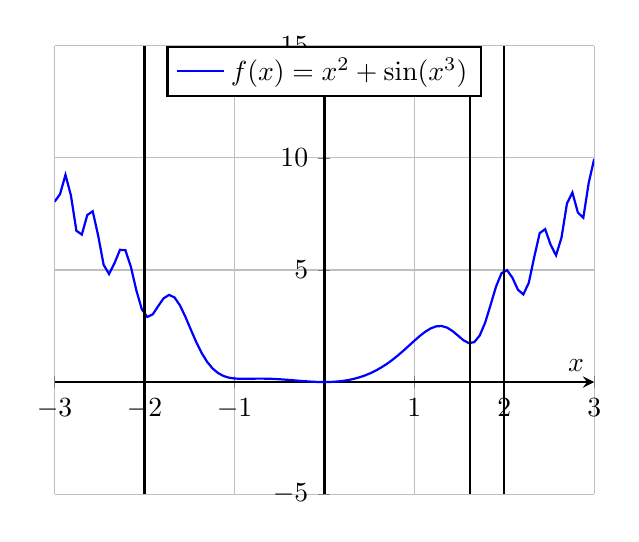
\begin{tikzpicture}
    \begin{axis}[
      domain=-3:3, % Domain of the plot
      samples=100, % Number of points to plot
      axis lines=middle, % Draw x and y axis
      xlabel={$x$}, % Label x-axis
      ylabel={$f(x)$}, % Label y-axis
      grid=major, % Add grid lines
      thick, % Line thickness
      ymin=-5, ymax=15, % Y-axis range
      xmin=-3, xmax=3, % X-axis range
      legend style={at={(0.5,1)}, anchor=north} % Legend positioning
    ]
    % Function plot: f(x) = x^2 + sin(x^3)
    \addplot[blue, thick] {x^2 + sin(deg(x^3))};
    \addlegendentry{$f(x) = x^2 + \sin(x^3)$}

    % Vertical line at x = -2
    \addplot[solid, black, thick] coordinates {(-2,-5) (-2,15)};

    % Vertical line at x = 2
    \addplot[solid, black, thick] coordinates {(2,-5) (2,15)};

    % Vertical line at x = 1.4
    \addplot[solid, black, thick] coordinates {(1.62,-5) (1.62,15)};
    \end{axis}
  \end{tikzpicture}

  \caption{Graph of $x^2 + sin(x^3)$ depicting an annealing schedule where gradient descent will converge to a local optimum instead of a global one.}\label{fig:annealing}
\end{figure}
